\subsection{Electromagnetic Waves: Definitions and Properties}
\label{subsec:ac-basics2}

Let's dive into the fascinating world of electromagnetic waves! These waves are the backbone of radio technology, traveling through space at approximately 300,000,000 meters per second - fast enough to circle the Earth about 7.5 times in one second! At their core, electromagnetic waves are composed of two primary components: the electric field and the magnetic field. These fields are perpendicular to each other and to the direction of wave propagation, as illustrated in Figure \ref{fig:em-wave}. Imagine them as two dancers moving in perfect harmony, each influencing the other.

\begin{figure}[h]
    \centering
    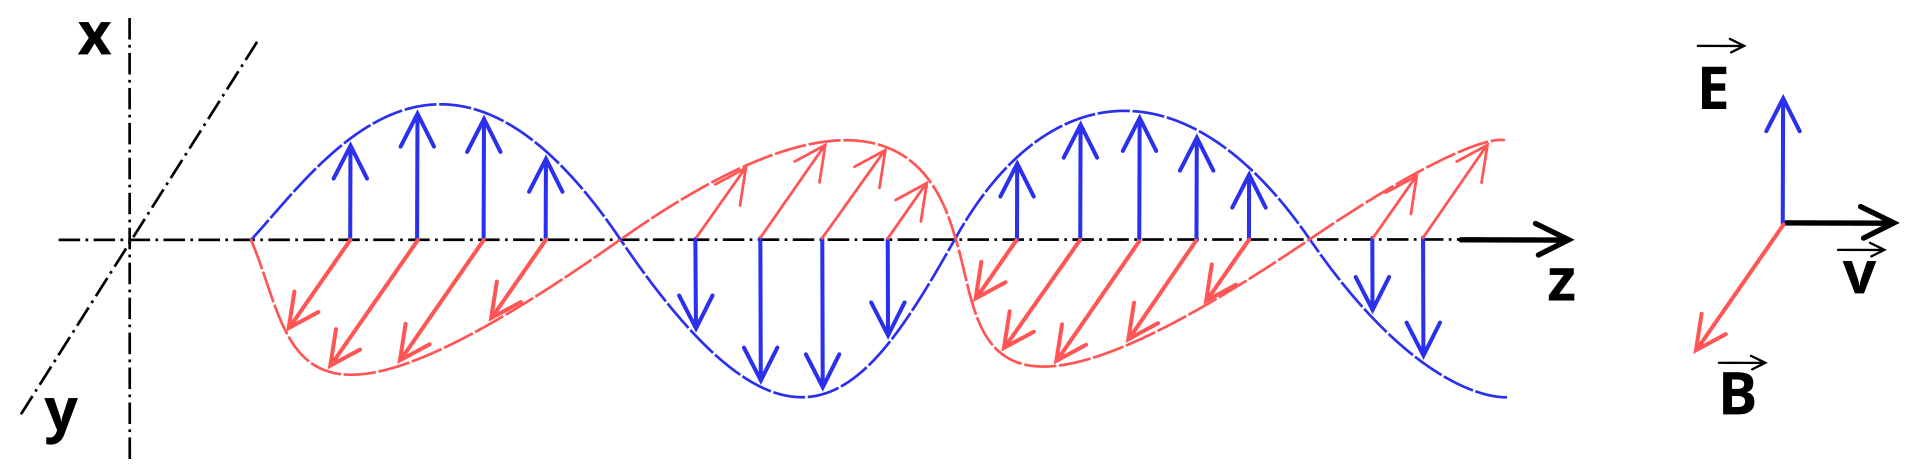
\includegraphics[width=0.8\textwidth]{tech/images/em-wave.png}
    \caption{Relationship between electric and magnetic fields in an electromagnetic wave. The electric field (E) and magnetic field (B) are perpendicular to each other and to the direction of wave propagation. As one field increases, the other follows 90 degrees later in space (like a synchronized dance where one partner bows while the other steps sideways). The wave's energy alternates between electric and magnetic fields as it travels through space, with both fields reaching their maximum and minimum values at different points.}
    \label{fig:em-wave}
\end{figure}

Maxwell's equations describe four fundamental relationships in electromagnetism (and they're like the superhero team of physics - each one has its own special power!):
\begin{itemize}[noitemsep]
    \item How electric charges create electric fields (Captain Electric's origin story)
    \item How magnetic fields are created by moving charges and changing electric fields (The Magnetic Marvel's secret technique)
    \item How magnetic fields circulate around electric currents and changing electric fields (The Dynamic Duo's team-up move)
    \item How magnetic poles always come in pairs - nature's way of saying "you complete me" (no lonely magnetic monopoles allowed!)
\end{itemize}

\subsection{Frequency and Wavelength}
The relationship between wavelength and frequency is inverse - as one increases, the other decreases. This relationship is described by the equation:

\begin{equation}
\lambda = \frac{c}{f}
\label{eq:wavelength}
\end{equation}

where \(\lambda\) is the wavelength in meters, \(c\) is the speed of light (approximately 300,000,000 meters per second), and \(f\) is the frequency in hertz. For example, if you have a frequency of 150 MHz, the wavelength would be:

\[
\lambda = \frac{300,000,000}{150,000,000} = 2 \text{ meters}
\]

The unit of frequency is the hertz (Hz), named after Heinrich Hertz, who first demonstrated the existence of electromagnetic waves. One hertz represents one cycle per second.

\subsection{Polarization}
Polarization refers to the orientation of the electric field as the wave travels. If the electric field oscillates in a single plane, the wave is said to be linearly polarized. If the electric field rotates as the wave propagates, it can be circularly or elliptically polarized. The orientation of the electric field determines the polarization state, which is crucial for applications like satellite communication and radar systems. These different types of polarization are shown in Figure \ref{fig:polarization}.

\begin{figure}[h]
    \centering
    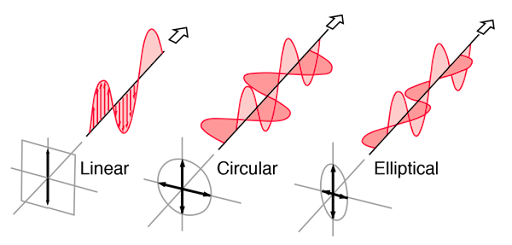
\includegraphics[width=0.8\textwidth]{tech/images/polarization.png}
    \caption{Radio wave polarization determined by the orientation of the electric field. Linear polarization occurs when the electric field oscillates in a single fixed plane (like a jump rope moving up and down). Circular polarization happens when the electric field rotates uniformly around the direction of propagation (like a spiral staircase). Elliptical polarization is similar to circular, but the field strength varies during rotation.}
    \label{fig:polarization}
\end{figure}

\subsection{Radio Frequency Bands}
Amateur radio bands are often identified by both their frequency and their approximate wavelength. For instance, the 2-meter band is a popular VHF band used by amateur radio operators. The major frequency bands are:

\begin{table}[h]
    \centering
    \begin{tabular}{|c|c|c|}
        \hline
        \textbf{Band} & \textbf{Frequency Range} & \textbf{Wavelength Range} \\
        \hline
        HF & 3 MHz to 30 MHz & 100 m to 10 m \\
        VHF & 30 MHz to 300 MHz & 10 m to 1 m \\
        UHF & 300 MHz to 3 GHz & 1 m to 10 cm \\
        SHF & 3 GHz to 30 GHz & 10 cm to 1 cm \\
        EHF & 30 GHz to 300 GHz & 1 cm to 1 mm \\
        \hline
    \end{tabular}
    \caption{Frequency and wavelength ranges for radio frequency bands.}
    \label{tab:frequency-ranges}
\end{table}

\subsubsection*{Questions}

\begin{tcolorbox}[colback=gray!10!white,colframe=black!75!black,title={T3B01}]
What is the relationship between the electric and magnetic fields of an electromagnetic wave?
\begin{enumerate}[label=\Alph*),noitemsep]
    \item They travel at different speeds
    \item They are in parallel
    \item They revolve in opposite directions
    \item \textbf{They are at right angles}
\end{enumerate}
\end{tcolorbox}

The electric and magnetic fields of an electromagnetic wave are perpendicular to each other and to the direction of wave propagation. This orthogonal relationship is fundamental to the nature of electromagnetic waves.

\begin{tcolorbox}[colback=gray!10!white,colframe=black!75!black,title={T3B02}]
What property of a radio wave defines its polarization?
\begin{enumerate}[label=\Alph*),noitemsep]
    \item \textbf{The orientation of the electric field}
    \item The orientation of the magnetic field
    \item The ratio of the energy in the magnetic field to the energy in the electric field
    \item The ratio of the velocity to the wavelength
\end{enumerate}
\end{tcolorbox}

Polarization refers to the orientation of the electric field of the radio wave. This orientation can be horizontal, vertical, or circular, depending on the application.

\begin{tcolorbox}[colback=gray!10!white,colframe=black!75!black,title={T3B03}]
What are the two components of a radio wave?
\begin{enumerate}[label=\Alph*),noitemsep]
    \item Impedance and reactance
    \item Voltage and current
    \item \textbf{Electric and magnetic fields}
    \item Ionizing and non-ionizing radiation
\end{enumerate}
\end{tcolorbox}

A radio wave consists of oscillating electric and magnetic fields. These fields propagate through space, carrying energy and information.

\begin{tcolorbox}[colback=gray!10!white,colframe=black!75!black,title={T3B04}]
What is the velocity of a radio wave traveling through free space?
\begin{enumerate}[label=\Alph*),noitemsep]
    \item \textbf{Speed of light}
    \item Speed of sound
    \item Speed inversely proportional to its wavelength
    \item Speed that increases as the frequency increases
\end{enumerate}
\end{tcolorbox}

In free space, radio waves travel at the speed of light, which is approximately 300,000,000 meters per second.

\begin{tcolorbox}[colback=gray!10!white,colframe=black!75!black,title={T3B05}]
What is the relationship between wavelength and frequency?
\begin{enumerate}[label=\Alph*),noitemsep]
    \item Wavelength gets longer as frequency increases
    \item \textbf{Wavelength gets shorter as frequency increases}
    \item Wavelength and frequency are unrelated
    \item Wavelength and frequency increase as path length increases
\end{enumerate}
\end{tcolorbox}

Wavelength and frequency are inversely related. As frequency increases, wavelength decreases, and vice versa.

\begin{tcolorbox}[colback=gray!10!white,colframe=black!75!black,title={T3B06}]
What is the formula for converting frequency to approximate wavelength in meters?
\begin{enumerate}[label=\Alph*),noitemsep]
    \item Wavelength in meters equals frequency in hertz multiplied by 300
    \item Wavelength in meters equals frequency in hertz divided by 300
    \item Wavelength in meters equals frequency in megahertz divided by 300
    \item \textbf{Wavelength in meters equals 300 divided by frequency in megahertz}
\end{enumerate}
\end{tcolorbox}

The formula \(\lambda = \frac{300}{f}\) (where \(f\) is in MHz) is a quick way to estimate wavelength in meters.

\begin{tcolorbox}[colback=gray!10!white,colframe=black!75!black,title={T3B07}]
In addition to frequency, which of the following is used to identify amateur radio bands?
\begin{enumerate}[label=\Alph*),noitemsep]
    \item \textbf{The approximate wavelength in meters}
    \item Traditional letter/number designators
    \item Channel numbers
    \item All these choices are correct
\end{enumerate}
\end{tcolorbox}

Amateur radio bands are often identified by their approximate wavelength in meters, which helps in understanding their practical use.

\begin{tcolorbox}[colback=gray!10!white,colframe=black!75!black,title={T3B08}]
What frequency range is referred to as VHF?
\begin{enumerate}[label=\Alph*),noitemsep]
    \item 30 kHz to 300 kHz
    \item \textbf{30 MHz to 300 MHz}
    \item 300 kHz to 3000 kHz
    \item 300 MHz to 3000 MHz
\end{enumerate}
\end{tcolorbox}

VHF stands for Very High Frequency and covers the range from 30 MHz to 300 MHz.

\begin{tcolorbox}[colback=gray!10!white,colframe=black!75!black,title={T3B09}]
What frequency range is referred to as UHF?
\begin{enumerate}[label=\Alph*),noitemsep]
    \item 30 to 300 kHz
    \item 30 to 300 MHz
    \item 300 to 3000 kHz
    \item \textbf{300 to 3000 MHz}
\end{enumerate}
\end{tcolorbox}

UHF, or Ultra High Frequency, ranges from 300 MHz to 3000 MHz.

\begin{tcolorbox}[colback=gray!10!white,colframe=black!75!black,title={T3B10}]
What frequency range is referred to as HF?
\begin{enumerate}[label=\Alph*),noitemsep]
    \item 300 to 3000 MHz
    \item 30 to 300 MHz
    \item \textbf{3 to 30 MHz}
    \item 300 to 3000 kHz
\end{enumerate}
\end{tcolorbox}

HF, or High Frequency, spans from 3 MHz to 30 MHz and is known for its long-distance communication capabilities.

\begin{tcolorbox}[colback=gray!10!white,colframe=black!75!black,title={T3B11}]
What is the approximate velocity of a radio wave in free space?
\begin{enumerate}[label=\Alph*),noitemsep]
    \item 150,000 meters per second
    \item \textbf{300,000,000 meters per second}
    \item 300,000,000 miles per hour
    \item 150,000 miles per hour
\end{enumerate}
\end{tcolorbox}

Radio waves travel at the speed of light, which is approximately 300,000,000 meters per second in free space.

\begin{tcolorbox}[colback=gray!10!white,colframe=black!75!black,title={T5A06}]
What is the unit of frequency?
\begin{enumerate}[label=\Alph*),noitemsep]
    \item \textbf{Hertz}
    \item Henry
    \item Farad
    \item Tesla
\end{enumerate}
\end{tcolorbox}

The unit of frequency is the hertz (Hz), named after Heinrich Hertz.

\begin{tcolorbox}[colback=gray!10!white,colframe=black!75!black,title={T5A12}]
What describes the number of times per second that an alternating current makes a complete cycle?
\begin{enumerate}[label=\Alph*),noitemsep]
    \item Pulse rate
    \item Speed
    \item Wavelength
    \item \textbf{Frequency}
\end{enumerate}
\end{tcolorbox}

Frequency is the term used to describe how many times per second an alternating current completes a full cycle.
